\section{65 - MAT - WS 2.1, WS 3.4, WS 2.3 - Roulette - Matura 2015/16 1. Nebentermin}

\begin{langesbeispiel} \item[0] %PUNKTE DES BEISPIELS
	
Beim Glücksspiel \textit{Roulette} versucht man, diejenige Zahl bzw. Gruppe von Zahlen zu erraten, die durch den Wurf einer Kugel in die Roulettemaschine bestimmt wird. 

Beim \textit{französischen Roulette} besteht die Roulettemaschine aus einer in eine Schüssel eingelassenen, drehbaren Scheibe mit 36 abwechselnd roten und schwarzen Nummernfächern sowie einem 37., grün gekennzeichneten Fach für die Null (vgl. Abbildung 1). Die Roulettescheibe wird in Bewegung gesetzt und die Kugel wird gegen die Drehrichtung in die Roulettemaschine geworfen. Dabei wird kein Nummernfach bevorzugt und es gibt keine Möglichkeit, das Ergebnis (etwa durch "`geschicktes"' Werfen) zu beeinflussen. 

Ziel ist es, in jedem einzelnen Spiel im Vorhinein zu erraten, in welchem Nummernfach die Kugel zu liegen kommen wird. 

Auf dem Spielfeld (vgl. Abbildung 2) werden die Spieleinsätze (Jetons) platziert. Beispielsweise sind die Felder mit der "`1"' und der "`7"' rot ("`rouge"'), die Felder mit der "`4"' und der "`6"' schwarz ("`noir"').

\meinlr{\resizebox{1\linewidth}{!}{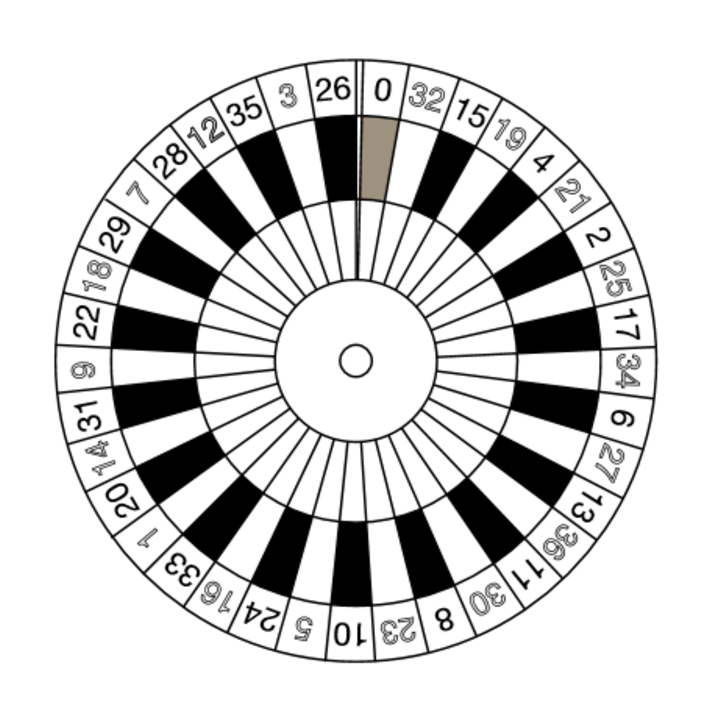
\includegraphics{../_database/Bilder/Bild65-1.eps}}

Abbildung 1

\begin{scriptsize}\begin{singlespace}Quelle:http://www.rouletteplay.com/images/\\
software\_logos\_small/european-roulette-wheel.gif [23.03.2016]\end{singlespace}\end{scriptsize}}{\resizebox{0.8\linewidth}{!}{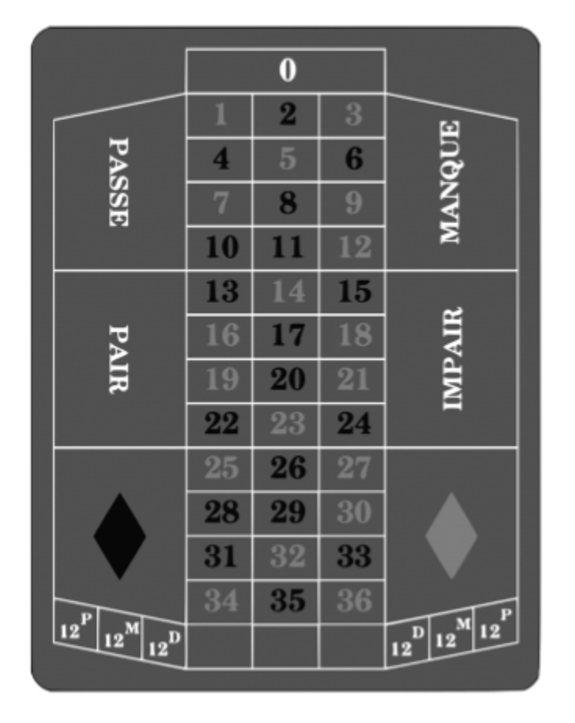
\includegraphics{../_database/Bilder/Bild65-2.eps}}

Abbildung 2

\begin{scriptsize}\begin{singlespace}Quelle:http://commons.wikimedia.org/wiki/\\
File:Roulette\_frz.png [23.03.2016]\end{singlespace}\end{scriptsize}}
 

\subsection{Aufgabenstellung:}
\begin{enumerate}
	\item Jemand argumentiert: "`Wenn die Kugel bei fünf Spielen hintereinander jedes Mal auf ein rotes Feld gefallen ist, fällt die Kugel beim 6. Spiel mit höherer Wahrscheinlichkeit auf ein schwarzes Feld als auf ein rotes, da bei einer längeren Spielserie dieselben Häufigkeiten für 'Rouge' und 'Noir' zu erwarten sind."' Gib an, ob diese Argumentation richtig oder falsch ist, und begründe deine Entscheidung!\leer
	
	An einem Roulettetisch werden an einem Abend 100 Spiele gespielt.
	
	\fbox{A} Berechne die Wahrscheinlichkeit, dass die Kugel dabei höchstens 40-mal in ein rotes Nummernfach fällt!\leer
	
	\item In der folgenden Tabelle sind einige Wettmöglichkeiten sowie die jeweiligen Gewinnquoten angeführt:\leer
	
	\begin{tabular}{|l|c|}\hline
	\cellcolor[gray]{0.9}Wettart&\cellcolor[gray]{0.9}Gewinnquote\\ \hline
	Rouge: Die Kugel fällt in ein rotes Nummernfach.&1:1\\ \hline
	Noir: Die Kugel fällt in ein schwarzes Nummernfach.&1:1\\ \hline
	$12^\text{P}$: erstes Dutzend (Zahlen 1 bis 12)&2:1\\ \hline
	$12^\text{M}$: mittleres Dutzend (Zahlen 13 bis 24)&2:1\\ \hline
	$12^\text{D}$: letztes Dutzend (Zahlen 25 bis 36)&2:1\\ \hline
	Plein: Man setzt auf eine der 37 Zahlen&35:1\\ \hline
	\multicolumn{1}{|p{10cm}|}{Cheval: Man setzt auf zwei auf dem Spielfeld horizontal oder vertikal benachbarte Zahlen, z.B. 2 und 5 oder 8 und 9.}&17:1\\ \hline	
	\end{tabular}\leer
	
 Eine Gewinnquote von $2:1$ bedeutet beispielsweise, dass im Falle eines Gewinns der Einsatz und zusätzlich das Doppelte des Einsatzes ausbezahlt wird. Im Falle eines Verlustes verliert man den Einsatz.

 Als Bankvorteil bezeichnet man bei Glücksspielen den erwarteten Verlust der Spielerin/des Spielers bezogen auf ihren/seinen Einsatz.

Eine Spielerin setzt \EUR{10} auf $12^\text{M}$. 

Berechne den Bankvorteil in Prozent des Einsatzes! 
 
Gib an, ob der in Prozent angegebene Bankvorteil größer wird, kleiner wird oder gleich bleibt, wenn die Spielerin/der Spieler bei einem Einsatz von \EUR{$a$} eine Cheval-Variante wählt!  

Begründe deine Entscheidung!


	
\end{enumerate}
\antwort{
\begin{enumerate}
	\item \subsection{Lösungserwartung:} 
	
Die Argumentation ist falsch. Da die einzelnen Spiele unabhängig voneinander sind, gilt auch für das sechste Spiel (unabhängig von den vorherigen Spielausgängen):

$P(\text{"`Rouge"'})=P(\text{"`Noir"'})=\frac{18}{37}$\leer

Mögliche Berechnung (z.B. durch Approximation durch die Normalverteilung ohne Stetigkeitskorrektur):  

Die binomialverteilte Zufallsvariable $X$ beschreibt, wie oft die Kugel in ein rotes Nummernfach fällt.

$n=100, p=\frac{18}{37}$

$P(X\leq 40)\approx 0,0418$ 

	\subsection{Lösungsschlüssel:}
	\begin{itemize}
		\item  Ein Punkt für die Angabe, dass die Argumentation nicht richtig ist, und für eine (sinngemäß) korrekte Begründung.
		\item  Ein Ausgleichspunkt für die richtige Lösung, wobei Ergebnisse durch Berechnung mit Stetigkeitskorrektur oder exakt mittels Binomialverteilung ebenfalls als richtig zu werten sind. Andere Schreibweisen des Ergebnisses (in Prozent) sind ebenfalls als richtig zu werten. 
		
		Toleranzintervall: $[0,03; 0,06]$  
		
		Die Aufgabe ist auch dann als richtig gelöst zu werten, wenn bei korrektem Ansatz das Ergebnis aufgrund eines Rechenfehlers nicht richtig ist. 
	\end{itemize}
	
	\item \subsection{Lösungserwartung:}
			
	Mögliche Berechnung:
	
	Bei $12^\text{M}$ erhält die Spielerin bei einem Einsatz von \EUR{10} mit der Wahrscheinlichkeit $\frac{12}{37}$ einen Gewinn von \EUR{20}.
	
	$\frac{12}{37}\cdot 20-\frac{25}{37}\cdot 10\approx -0,27$
	
	D.h., der erwartete Verlust beträgt ca. \EUR{0,27}.
	
	Bankvorteil: \EUR{0,27} bzw. 2,7\,\% des Einsatzes\leer
	
	Cheval bei einem Einsatz von \EUR{$a$}:
	
	erwarteter Gewinn: $\frac{2}{37}\cdot 17\cdot a-\frac{35}{37}\cdot a=-\frac{1}{37}\cdot a\approx -0,027\cdot a$
	
	Der Bankvorteil bleibt mit ca. 2,7\,\% des Einsatzes gleich.
	
	\subsection{Lösungsschlüssel:}
	
\begin{itemize}
	\item Ein Punkt für die richtige Lösung, wobei diese sowohl in Prozentangabe als auch als Geldbetrag als richtig zu werten ist. 
	
	Toleranzintervall: [\EUR{0,27}; \EUR{0,30}] bzw. $[2,7\,\%; 3\,\%]$ 
	\item Ein Punkt für die Angabe, dass der Bankvorteil gleich bleibt, und für eine (sinngemäß) korrekte Begründung.  
\end{itemize}

\end{enumerate}}
		\end{langesbeispiel}